\documentclass{article}
\usepackage[MeX]{polski}
\usepackage[utf8]{inputenc}
\usepackage{graphicx}
\usepackage{adjustbox}
\title{Przerzutnik JK}
\begin{document}
\maketitle
\section{O przerzutniku}
{\centering
\begin{tabular}{|c|c|c|c|c|}\hline
\rule{10pt}{0pt} & \rule{10pt}{0pt} & \rule{10pt}{0pt} & \rule{10pt}{0pt} & \rule{10pt}{1pt}\\
CLK & J&K&Q&Q\\ \hline
\rule{10pt}{0pt} & \rule{10pt}{0pt} & \rule{10pt}{0pt} & \rule{10pt}{0pt} & \rule{10pt}{1pt}\\
0->1 & 0 & 0 & Q&Q\\  \hline
0->1 & 0 & 1 & 0 &1\\ \hline
0->1 & 1 & 0 & 1 & 0\\ \hline
\rule{10pt}{0pt} & \rule{10pt}{0pt} & \rule{10pt}{0pt} & \rule{10pt}{1pt} & \rule{10pt}{0pt}\\
0->1 & 1 & 1 & Q & Q\\ \hline
\end{tabular}
\par
}
Tablica prawdy pokazuje, jaka wartość będzie na wyjsciu przerzutnika(Q) w zalezności od jego wejść J i K oraz sygnału zegarowego CLK. Wartość 1 oznacza stan wysoki, a wartość 0 stan niski. Przerzutnik pracuje w takt zegara, kiedy zmienia się zbocze sygnału zegarowego, czyli kiedy wartość zmienia się z 0 na 1.
\section{Krok po kroku}
\begin{enumerate}
\item Ze strony pobrać plik flipflop.
\item Należy uruchomić program Xilinx ISE 10.1
\item Utworzyć nowy projekt poprzez File/New Project. Upewnić się, że został wybrany folder taki jak na rysunku. Podać nazwę projektu i wybrać z rozwijanego menu Schematic\\ \begin{minipage}[t]{\linewidth}
          \raggedright
          \adjustbox{valign=t}{%
            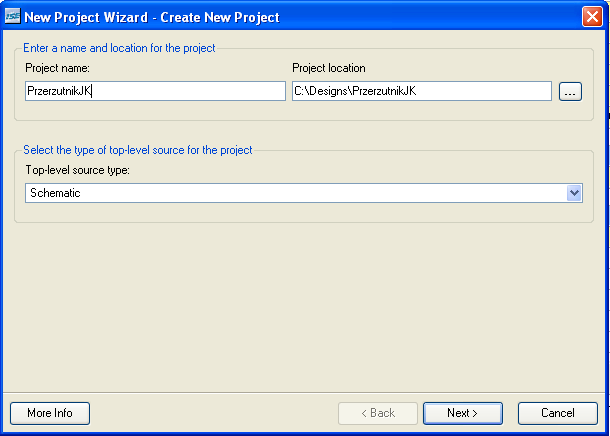
\includegraphics[width=1\linewidth]{1.PNG}%
          }

          \medskip
          Nacisnąć przycisk Next, a następnie ustawić parametry tak jak na rysunku.
	\adjustbox{valign=t}{%
            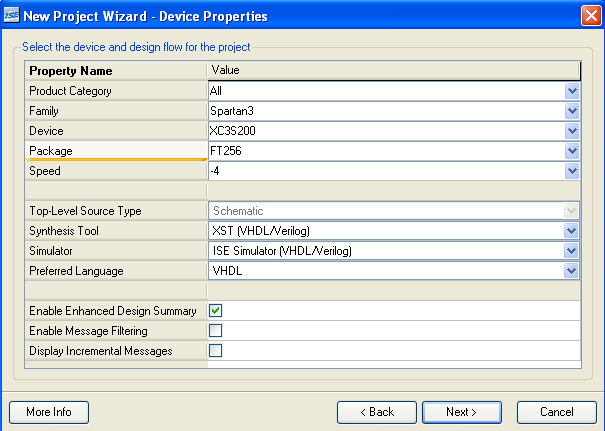
\includegraphics[width=1\linewidth]{2.PNG}%
          }
	Nacisnąć przycisk Next. Następnie nacisnąć Add Source i wybrać pobrane wcześniej pliki. Następnie nacisnąć kolejne przyciski Next i Finish.
    \end{minipage}
\item Następnie należy utworzyć plik symulacyjny Testbench. Dzięki temu będzie można przetestować zaprojektowany układ przed zaprogramowaniem urządzenia docelowego. Aby to uczynić należy nacisnąć prawy przycisk mysz w miejscu zaznaczonym jak na rysunku i następnie wybrać opcję New Source. W wyświetlonym oknie wybrać opcje tak jak na rysunku i nadać nazwę pliku. \\ \begin{minipage}[t]{\linewidth}
          \raggedright
          \adjustbox{valign=t}{%
            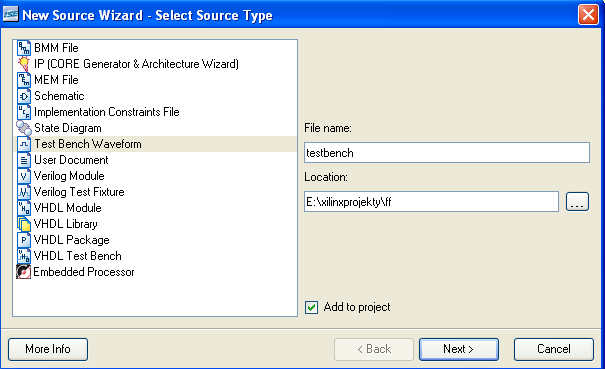
\includegraphics[width=1\linewidth]{4.PNG}%
          }

          \medskip
Następnie nacisnąć dwukrotnie przycisk Next oraz na koniec Finish. Wyskoczy kolejne okienko w którym można zmienić parametry zegara takie jak np. jego okres, należy nacisnąć przycisk Finish.
 \end{minipage}
\item Można dowolnie ustawić sygnały J oraz K za które odpowiedzialne są przyciski 0 oraz 1. Przycisk 2 służy do resetowania ukladu. Sygnał zmienia się poprzez naciśnięcie na wykresie czasowym w miejscu w którym chcemy aby nastąpiła zmiana.\\ \begin{minipage}[t]{\linewidth}
          \raggedright
          \adjustbox{valign=t}{%
            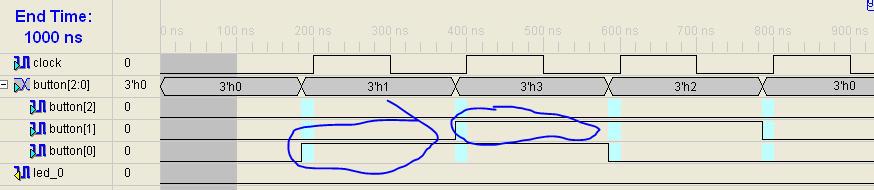
\includegraphics[width=1\linewidth]{5.PNG}%
          }

          \medskip
Na rysunku zaznaczono miejsca kliknięć.
 \end{minipage}
\item Należy uruchomić symulację poprzez przejście do menu Sources oraz Processes, tak jak zaznaczono na rysunku. A następnie wybranie Behavioral simulation, zaznaczenie pliku Testbench oraz rozpoczęcie symulacji przez dwukrotne kliknięcie we wskazanym miejscu.\\ \begin{minipage}[t]{\linewidth}
          \raggedright
          \adjustbox{valign=t}{%
            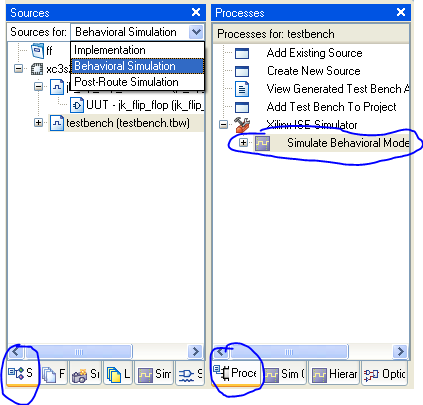
\includegraphics[width=1\linewidth]{6.PNG}%
          }

          \medskip
 \end{minipage}
\item Jesli wszystko działa poprawnie można przejść do testowania układu bezpośrednio na płytce. Aby to zrobić w okienku Sources należy przejsć do menu Implentation i zaznaczyć nazwę pliku. W okienku Processes należy dwukrotnie nacisnąć Configure Target Device.\\ \begin{minipage}[t]{\linewidth}
          \raggedright
          \adjustbox{valign=t}{%
            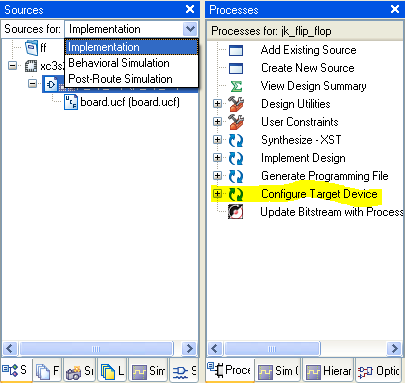
\includegraphics[width=1\linewidth]{7.PNG}%
          }

          \medskip
Zatwierdzić wywietlony komunikat przyciskiem Ok, a następnie nacisnąć przycisk Finish. W wyświetlonym oknie nalezż wybrać plik z rozszerzeniem .bit i nacisnąć przycisk Open, a w kolejnym nacisnąć Bypass. W okienku które wyskoczy naciskamy przycisk Ok. Ostatnim krokiem jest naciśnięcie prawym przyciskiem w miejscu jak na rysunku oraz wybrać opcję Program.
\adjustbox{valign=t}{%
            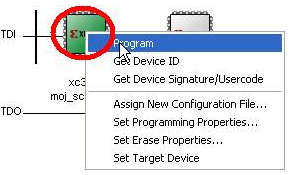
\includegraphics[width=1\linewidth]{8.PNG}%
          }
 \end{minipage}
\item Można zaobserbować świecenenie diody poprzez naciskanie roznych kombinacji przyciskow, zgodnie z tablicą prawdy przerzutnika JK.
\end{enumerate}
\end{document}